% % % % % % % % % % % % % % % % % % % % % % % % % % % % % % % % % % % % % % % %
% LaTeX4EI Template for Cheat Sheets                                Version 1.1
%
% Authors: Emanuel Regnath, Martin Zellner
% Contact: info@latex4ei.de
% Encode: UTF-8, tabwidth = 4, newline = LF
% % % % % % % % % % % % % % % % % % % % % % % % % % % % % % % % % % % % % % % %


% ======================================================================
% Document Settings
% ======================================================================

% possible options: color/nocolor, english/german, threecolumn
% defaults: color, english
\documentclass[english]{latex4ei/latex4ei_sheet}
\usepackage{amsmath}
\usepackage{empheq}
\usepackage{gensymb}
\usepackage{tikz}
\usetikzlibrary{arrows.meta,calc,angles,positioning}

\def\centerarc[#1](#2)(#3:#4:#5)
% Syntax: [draw options] (center) (initial angle:final angle:radius)
{ \draw[#1] ($(#2)+({#5*cos(#3)},{#5*sin(#3)})$) arc (#3:#4:#5); }

% set document information
\title{LaTeX4EI \\ Cheat Sheet}
\author{LaTeX4EI}					% optional, delete if unchanged
\myemail{info@latex4ei.de}			% optional, delete if unchanged
\mywebsite{www.latex4ei.de}			% optional, delete if unchanged


% ======================================================================
% Begin
% ======================================================================
\begin{document}

% Title
% ----------------------------------------------------------------------
\maketitle   % requires ./img/Logo.pdf

% Section
% ----------------------------------------------------------------------

\section{Einheiten}

\begin{sectionbox}
	\subsection{SI-Präfixe}
	
	\begin{tablebox}{ccl|ccl}
		Symbol & Präfix & Faktor & Symbol & Präfix & Faktor \\
		\hline
		Q  & Quetta & $10^{30}$ & d & Dezi & $10^{-1}$\\
		R  & Ronna  & $10^{27}$ & c & Zenti & $10^{-2}$\\
		Y  & Yotta  & $10^{24}$ & m & Milli & $10^{-3}$\\
		Z  & Zetta  & $10^{21}$ & µ & Mikro & $10^{-6}$\\ 
		E  & Exa    & $10^{18}$ & n & Nano  & $10^{-9}$\\
		P  & Peta   & $10^{15}$ & p & Piko  & $10^{-12}$\\
		T  & Tera   & $10^{12}$ & f & Femto  & $10^{-15}$\\
	 	G  & Giga   & $10^9$    & a & Atto   & $10^{-18}$\\
		M  & Mega   & $10^6$    & z & Zepto  & $10^{-21}$\\
		k  & Kilo   & $10^3$    & y & Yokto  & $10^{-24}$\\
		h  & Hekto  & $10^2$    & r & Ronto  & $10^{-27}$\\
		da & Deka   & $10^1$    & q & Quekto & $10^{-30}$\\
	\end{tablebox}

	\subsection{Binäre Präfixe}
	
	\begin{tablebox}{ccll}
		Symbol & Präfix & Faktor & Dez. Äquiv. \\
		\hline			
		Ki & Kibi  & $2^{10}$  & $= 1.024e3$ \\
		Mi & Mebi  & $2^{20}$  & $≈ 1.049e6$ \\
		Gi & Gibi  & $2^{30}$  & $≈ 1.074e9$ \\
		Ti & Tebi  & $2^{40}$  & $≈ 1.100e12$ \\
		Pi & Pebi  & $2^{50}$  & $≈ 1.126e15$ \\
		Ei & Exbi  & $2^{60}$  & $≈ 1.152e18$ \\
		Zi & Zebi  & $2^{70}$  & $≈ 1.181e21$ \\
		Yi & Yobi  & $2^{80}$  & $≈ 1.209e24$ \\
		Ri & Robi  & $2^{90}$  & $≈ 1.238e27$ \\
		Qi & Quebi & $2^{100}$ & $≈ 1.268e30$ \\
	\end{tablebox}

	\subsection{SI-Einheiten}

	\begin{tablebox}{llc}
		Grösse & Einheit & \\
		\hline
		Länge & Meter & m \\
		Masse & Kilogramm & kg \\
		Zeit & Sekunde & s \\
		Stromstärke & Ampere & A \\
		Temperatur & Kelvin & K \\
		Stoffmenge & - & mol \\
		Lichtstärke & Candela & cd			
	\end{tablebox}	
	
	\subsection{Abgeleitete Einheiten}

	\begin{tablebox}{lcllc}
		Grösse & Sym. & Einheit &  & SI \\
		\hline
		Kraft & F & Newton & N & $kg\cdot m/s^2$ \\
		Energie/Arbeit & E/W & Joule & J & $Nm$ \\
		Leistung & P & Watt & W & $J/s$ \\
		El. Ladung & Q & Coulomb & C & $A \cdot s$ \\
		El. Potential & $\phi$ & Volt & V & $J/C$ \\
		Spannung & U & Volt & V & $J/C$ \\
		El. Widerstand & R & Ohm & $\ohm$ & $V/A$ \\
		El. Leitwert & G & Siemens & S & $A/V$ \\
		Spez. el. Widerstand & $\rho$ & - & - & $Ωm$ \\
		Spez. el. Leitwert & $\gamma$ & - & - & $S/m$ \\
		El. Feldstärke & E & - & - & $V/m$ \\
		El. Stromdichte & J & - & - & $A/m^2$ \\
	\end{tablebox}
		
\end{sectionbox}

\begin{sectionbox}
	Summe:
	\begin{emphbox}
		$\sum\limits_{k=m}^{n}a_k = \sum\limits_{m≤k≤n}^{}a_k = a_m + a_{m+1} + \ldots + a_n $
		
		$ \sum\limits_{k=m}^{n}(a_k+b_k) = \sum\limits_{k=m}^{n}a_k + \sum\limits_{k=m}^{n}b_k $
	\end{emphbox}
\end{sectionbox}	
	
\section{Elektrotechnik}

\subsection{Widerstandfarbcodes}
	3 oder 4 Ringe: Z-E-M-T \\
	5 oder 6 Ringe: H-Z-E-M-T-TK \\
	\#: H/Hunderter (100x), Z/Zehner (10x), E/Einer (1x) \\
	M: Multiplikator, T: Toleranz, TK: Temperaturkoeffizient
	\begin{tablebox*}{lllll}
		Farbe & \# & Mult. & Tol. & TK \\
		\hline
		ohne    &   &                        & $\pm 20\%$   & \\
		silber  &   & $10^{-2}$ = 0.01       & $\pm 10\%$   & \\
		gold    &   & $10^{-1}$ = 0.1        & $\pm 5\%$    & \\
		schwarz & 0 & $10^0$ = 1             &              & $200 \cdot 10^{-6}/K$ \\			
		braun   & 1 & $10^1$ = 10            & $\pm 1\%$    & $100 \cdot 10^{-6}/K$ \\
		rot     & 2 & $10^2$ = 100           & $\pm 2\%$    & $50 \cdot 10^{-6}/K$\\
		orange  & 3 & $10^3$ = 1000          &              & $15 \cdot 10^{-6}/K$ \\
		gelb    & 4 & $10^4$ = 10'000        &              & $25 \cdot 10^{-6}/K$ \\
		grün    & 5 & $10^5$ = 100'000       & $\pm 0.5\%$  & \\
		blau    & 6 & $10^6$ = 1'000'000     & $\pm 0.25\%$ & $10 \cdot 10^{-6}/K$ \\
		violett & 7 & $10^7$ = 10'000'000    & $\pm 0.1\%$  & $5 \cdot 10^{-6}/K$ \\
		grau    & 8 & $10^8$ = 100'000'000   & $\pm 0.05\%$ & \\
		weiss   & 9 & $10^9$ = 1'000'000'000 &              & \\
	\end{tablebox*}

\subsection{E-Reihen}
	\begin{tablebox*}{llllllll}
			\multicolumn{8}{l}{E3 (40\% Toleranz)}  \\
			\hline
			1.0 & 2.2 & 4.7 & & & & & \\
			\multicolumn{8}{l}{E6 (20\% Toleranz)}  \\
			\hline
			1.0 & 1.5 & 2.2 & 3.3 & 4.7 & 6.8 \\
			\multicolumn{8}{l}{E12 (10\% Toleranz)}  \\
			\hline
			1.0 & 1.2 & 1.5 & 1.8 & 2.2 & 2.7 \\
			3.3 & 3.9 & 4.7 & 5.6 & 6.8 & 8.2 \\
			\multicolumn{8}{l}{E24 (5\% Toleranz)}  \\
			\hline
			1.0 & 1.1 & 1.2 & 1.3 & 1.5 & 1.6 & 1.8 & 2.0 \\
			2.2 & 2.4 & 2.7 & 3.0 & 3.3 & 3.6 & 3.9 & 4.3 \\
			4.7 & 5.1 & 5.6 & 6.2 & 6.8 & 7.5 & 8.2 & 9.1 \\
			\multicolumn{8}{l}{E48 (2\% Toleranz)}  \\
			\hline
			1.00 & 1.05 & 1.10 & 1.15 & 1.21 & 1.27 & 1.33 & 1.40 \\
			1.47 & 1.54 & 1.62 & 1.69 & 1.78 & 1.87 & 1.96 & 2.05 \\
			2.15 & 2.26 & 2.37 & 2.49 & 2.61 & 2.74 & 2.87 & 3.01 \\
			3.16 & 3.32 & 3.48 & 3.65 & 3.83 & 4.02 & 4.22 & 4.42 \\
			4.64 & 4.87 & 5.11 & 5.36 & 5.62 & 5.90 & 6.19 & 6.49 \\
			6.81 & 7.15 & 7.50 & 7.87 & 8.25 & 8.66 & 9.09 & 9.53 \\
	\end{tablebox*}
	\begin{tablebox*}{llllllll}
			\multicolumn{8}{l}{E96 (1\% Toleranz)} \\
			\hline
			1.00 & 1.02 & 1.05 & 1.07 & 1.10 & 1.13 & 1.15 & 1.18 \\
			1.21 & 1.24 & 1.27 & 1.30 & 1.33 & 1.37 & 1.40 & 1.43 \\
			1.47 & 1.50 & 1.54 & 1.58 & 1.62 & 1.65 & 1.69 & 1.74 \\
			1.78 & 1.82 & 1.87 & 1.91 & 1.96 & 2.00 & 2.05 & 2.10 \\
			2.15 & 2.21 & 2.26 & 2.32 & 2.37 & 2.43 & 2.49 & 2.55 \\
			2.61 & 2.67 & 2.74 & 2.80 & 2.87 & 2.94 & 3.01 & 3.09 \\
			3.16 & 3.24 & 3.32 & 3.40 & 3.48 & 3.57 & 3.65 & 3.74 \\
			3.83 & 3.92 & 4.02 & 4.12 & 4.22 & 4.32 & 4.42 & 4.53 \\
			4.64 & 4.75 & 4.87 & 4.99 & 5.11 & 5.23 & 5.36 & 5.49 \\
			5.62 & 5.76 & 5.90 & 6.04 & 6.19 & 6.34 & 6.49 & 6.65 \\
			6.81 & 6.98 & 7.15 & 7.32 & 7.50 & 7.68 & 7.87 & 8.06 \\
			8.25 & 8.45 & 8.66 & 8.87 & 9.09 & 9.31 & 9.53 & 9.76 \\
			\multicolumn{8}{l}{E192 (0.5\% Toleranz und tiefer)} \\
			\hline
			1.00 & 1.01 & 1.02 & 1.04 & 1.05 & 1.06 & 1.07 & 1.09 \\
			1.10 & 1.11 & 1.13 & 1.14 & 1.15 & 1.17 & 1.18 & 1.20 \\
			1.21 & 1.23 & 1.24 & 1.26 & 1.27 & 1.29 & 1.30 & 1.32 \\
			1.33 & 1.35 & 1.37 & 1.38 & 1.40 & 1.42 & 1.43 & 1.45 \\
			1.47 & 1.49 & 1.50 & 1.52 & 1.54 & 1.56 & 1.58 & 1.60 \\
			1.62 & 1.64 & 1.65 & 1.67 & 1.69 & 1.72 & 1.74 & 1.76 \\
			1.78 & 1.80 & 1.82 & 1.84 & 1.87 & 1.89 & 1.91 & 1.93 \\
			1.96 & 1.98 & 2.00 & 2.03 & 2.05 & 2.08 & 2.10 & 2.13 \\
			2.15 & 2.18 & 2.21 & 2.23 & 2.26 & 2.29 & 2.32 & 2.34 \\
			2.37 & 2.40 & 2.43 & 2.46 & 2.49 & 2.52 & 2.55 & 2.58 \\
			2.61 & 2.64 & 2.67 & 2.71 & 2.74 & 2.77 & 2.80 & 2.84 \\
			2.87 & 2.91 & 2.94 & 2.98 & 3.01 & 3.05 & 3.09 & 3.12 \\
			3.16 & 3.20 & 3.24 & 3.28 & 3.32 & 3.36 & 3.40 & 3.44 \\
			3.48 & 3.52 & 3.57 & 3.61 & 3.65 & 3.70 & 3.74 & 3.79 \\
			3.83 & 3.88 & 3.92 & 3.97 & 4.02 & 4.07 & 4.12 & 4.17 \\
			4.22 & 4.27 & 4.32 & 4.37 & 4.42 & 4.48 & 4.53 & 4.59 \\
			4.64 & 4.70 & 4.75 & 4.81 & 4.87 & 4.93 & 4.99 & 5.05 \\
			5.11 & 5.17 & 5.23 & 5.30 & 5.36 & 5.42 & 5.49 & 5.56 \\
			5.62 & 5.69 & 5.76 & 5.83 & 5.90 & 5.97 & 6.04 & 6.12 \\
			6.19 & 6.26 & 6.34 & 6.42 & 6.49 & 6.57 & 6.65 & 6.73 \\
			6.81 & 6.90 & 6.98 & 7.06 & 7.15 & 7.23 & 7.32 & 7.41 \\
			7.50 & 7.59 & 7.68 & 7.77 & 7.87 & 7.96 & 8.06 & 8.16 \\
			8.25 & 8.35 & 8.45 & 8.56 & 8.66 & 8.76 & 8.87 & 8.98 \\
			9.09 & 9.20 & 9.31 & 9.42 & 9.53 & 9.65 & 9.76 & 9.88
	\end{tablebox*}
	
\begin{sectionbox}
	\subsection{Ohmsches Gesetz}

	\begin{emphbox}
	Ohmsches Gesetz: $ U = R \cdot I = \frac{I}{G} $
	\end{emphbox}

	\subsection{Leistung}

	\begin{emphbox}
	$ P = U \cdot I = \frac{U^2}{R} = I^2 \cdot R $
	\end{emphbox}
	

		
\end{sectionbox}

\begin{sectionbox}
	\subsection{Kirchoffsche Gesetze}

	Knotenregel:
	\begin{emphbox}
		In einem Knoten: Summe der zufliessenden Ströme = Summe der abfliessenden Ströme\\
		$\sum _{k=1}^{n}I_k = 0$
	\end{emphbox}
	
	Maschenregel:
	\begin{emphbox}
		In einer Masche: Summe der Teilspannungen addieren sich zu Null. Pfeilrichtungen beachten!\\
		$\sum _{k=1}^{n}U_k = 0$
	\end{emphbox}

\end{sectionbox}

\begin{sectionbox}
	\subsection{Strom}
	Elektronen bewegen sich entgegengesetzt zur Stromrichtung

	\begin{tabular}{cc}
	\parbox{1cm}{
		\begin{emphbox}
			\begin{align*}
				b &= \frac{v}{E} \\
				J &= \frac{I}{A}
			\end{align*}
		\end{emphbox}
	} & 
	
	\parbox{5cm}{
		\begin{symbolbox}
			$b$: Ladungsträgerbeweglichkeit (in $m^2/Vs$) \\
			$v$: Driftgeschwindigkeit (in m/s) \\
			$E$: el. Feldstärke (in V/m) \\
			$J$: Stromdichte \\
			$I$: Stromstärke \\
			$A$: Leiterquerschnitt
		\end{symbolbox}
	}
\end{tabular}

\end{sectionbox}

\begin{sectionbox}
	\subsection{Widerstand}

	\begin{tabular}{cc}
	\parbox{2.5cm}{
		\begin{emphbox}
			\begin{align*}
				R &= \frac{\rho \cdot l}{A} = \frac{l}{\gamma \cdot A} \\
				\gamma &= \frac{1}{\rho} \\
				R &= \frac{1}{G}
			\end{align*}
		\end{emphbox}
	} & 

	\parbox{3cm}{
		\begin{symbolbox}
			R: Widerstand (in \ohm) \\
			G: Leitwert (in S) \\
			$\rho$ : spez. Widerstand \\
			$\gamma$ : Leitfähigkeit \\
			A : Leiterquerschnitt \\
			l: Leiterlänge
		\end{symbolbox}
	}
	\end{tabular}

	\begin{emphbox}
	
		\begin{tabular}{l|l}
			Parallelschaltung & Serieschaltung \\
			%\hline
			$ \frac{1}{R_{tot}} = \sum\limits _{k=1}^{n}\frac{1}{R_k} $	&
			$ R_{tot} = \sum\limits _{k=1}^{n}R_k $ \\
			$ G_{tot} = \sum\limits _{k=1}^{n}G_k $ & \\
		\end{tabular}
	\end{emphbox}
	
\end{sectionbox}


\begin{sectionbox}
	\subsection{Kondensator}

	Lade-/Entladevorgang:
	\begin{emphbox}
		\begin{align*}
			u_C(t) &= U_0+ ΔU \cdot e^{-{\frac{t}{τ}}} = U_0+ (U_{C,t0}-U_0) \cdot e^{-{\frac{t}{τ}}} \\
			i_C(t) &= \frac{u_C(t)}{R_C} = \frac{U_0}{R_C}+\frac{ΔU}{R_C}\cdot e^{-{\frac{t}{τ}}}
		\end{align*}
	\end{emphbox}




\begin{emphbox}
	\begin{tabular}{l|l}
		Ladevorgang & Entladevorgang \\
		
		$ u_C(t) = U_0 \cdot (1-e^{-{\frac{t}{τ}}}) $ &
		$ u_C(t) = U_0 \cdot e^{-{\frac{t}{τ}}} $ \\

		$ i_C(t) = I_0 \cdot e^{-{\frac{t}{τ}}} $ &
		$ i_C(t) = -I_0 \cdot e^{-{\frac{t}{τ}}} $ \\
		
	\end{tabular}



\end{emphbox}

mit
\begin{emphbox}
	$I_0 = \frac{U_0}{R_C}$
	
	$τ = R_C \cdot C$
\end{emphbox}

	
\end{sectionbox}

\begin{sectionbox}
	\subsection{Spule}

	Lade-/Entladevorgang:
	\begin{emphbox}
		$u_C(t) = U_0+ ΔU \cdot e^{-{\frac{t}{τ}}} = U_0+ (U_{C,t0}-U_0) \cdot e^{-{\frac{t}{τ}}} ???$

		$i_C(t) = \frac{u_C(t)}{R_C} = \frac{U_0}{R_C}+\frac{ΔU}{R_C}\cdot e^{-{\frac{t}{τ}}} ???$
	\end{emphbox}

	\begin{emphbox}
		\begin{tabular}{l|l}
			Ladevorgang & Entladevorgang \\
			$u_L(t) = U_0 \cdot e^{-{\frac{t}{τ}}}$ &
			$u_L(t) = -U_0 \cdot e^{-{\frac{t}{τ}}}$ \\
			$i_L(t) = I_0 \cdot (1-e^{-{\frac{t}{τ}}})$ &
			$i_L(t) = I_0 \cdot e^{-{\frac{t}{τ}}}$ \\
		\end{tabular}
	\end{emphbox}

	mit: $I_0 = \frac{U_0}{R_L}, τ = \frac{L}{R_L}$	

	
\end{sectionbox}


\begin{sectionbox}
	\subsection{Phasenwinkel}

	\begin{emphbox}
		Kreisfrequenz: $\omega = 2\pi f = 2\pi/T$\\
		Phasenwinkel: $\varphi(t) = \omega t + \varphi_0$\\
		Kosinusform: $x(t) = \hat{x} \cos(\omega t + \varphi_0)$\\
	\end{emphbox}

		mit: f = Frequenz\\
		T = Periodendauer\\
		$\varphi_0$ = Nullphasenwinkel, Phasenwinkel zum Zeitpunkt t=0

\end{sectionbox}
	

\begin{sectionbox}
	\subsection{Phasor/komplexe Amplitude}
	Für harmonisch schwingende zeitabhängige Grössen:
	\begin{emphbox}
		$a(t) = \hat{a} \cos(\omega t + \varphi_0)$\\
	
	\end{emphbox}
\end{sectionbox}

\begin{sectionbox}
	\subsection{Frequenzgang}
	\begin{emphbox}
		Verstärkung/Dämpfung: $v = 20\log \frac{G}{G_0}$
	\end{emphbox}
	mit:
	$G$ : Grösse\\
	$G_0$ : Bezugsgrösse\\
	$[v]$ = dB
	
	Grenzfrequenz $f_g$ / Grenzkreisfrequenz $\omega_g$):
	Bei dieser Frequenz ist der Betrag einer frequenzabhängigen Grösse	um $\sqrt{2}$ grösser oder kleiner als eine konstante Bezugsgrösse.
	
	
	Dekade: lin.: $\cdot 10$ o. $/10$, log.: $\pm 20 \si{\dB}$\\
	Oktave:	lin.: $\cdot 2$ o. $/2$, log.: $\pm 6 \si{\dB}$
	\begin{emphbox}
		Normierte Frequenz: $\Omega = \frac{\omega}{\omega_g}$
	\end{emphbox}

\end{sectionbox}

\begin{sectionbox}
	



\end{sectionbox}
\section{Trigonometrie}

\begin{sectionbox}
	\subsection{Sinus}
		\begin{emphbox}
			\begin{align*}
			 \sin \alpha &= \frac{Gegenkathete}{Hypotenuse} \\
			 \sin (-\alpha) &= -\sin \alpha \\
			 \sin (90 \degree + \alpha) &= \sin (90 \degree - \alpha)
			\end{align*}
		\end{emphbox}
		ungerade Funktion
	\subsection{Cosinus}
		\begin{emphbox}
			\begin{align*}
			\cos \alpha &= \frac{Ankathete}{Hypotenuse}\\
			\cos (-\alpha) &= \cos \alpha\\
			\cos (90 \degree + \alpha) &= -\cos (90 \degree - \alpha)
			\end{align*}
		\end{emphbox}
		Gerade Funktion

	\subsection{Tangens}
		\begin{emphbox}
			\begin{align*}
			\tan \alpha &= \frac{Gegenkathete}{Ankathete} \\
			\tan \alpha &= \frac{\sin \alpha}{\cos \alpha} 
			\end{align*}
		\end{emphbox}
		
	\subsection{Cotangens}
		\begin{emphbox}
			\begin{align*}
			\cot \alpha &= \frac{Ankathete}{Gegenkathete} \\
			\cot \alpha &= \frac{\cos \alpha}{\sin \alpha} 		
			\end{align*}
		\end{emphbox}
	mit:\\
	a = Gegenkathete\\
	b = Ankathete\\
	c = Hypotenuse

	\begin{tikzpicture}
		\draw (0, 0) -- (3, 0) -- (2, 2) -- (0, 0);
		\coordinate[label=left:$A$] (A) at (0, 0);
		\coordinate[label=right:$B$] (B) at (3, 0);
		\coordinate[label=above:$C$] (C) at (2, 2);
	\end{tikzpicture}

	\subsection{Trigonometrischer Pythagoras}
		\begin{emphbox}
			$ \sin ^2 \alpha + \cos ^2 \alpha = 1 $
		\end{emphbox}
		
	\subsection{Sinussatz}
		\begin{emphbox}
			$ \frac{a}{\sin \alpha} = \frac{b}{\sin \beta} = \frac{c}{\sin \gamma} = \frac{a \cdot b \cdot c}{2 \cdot A} = 2 \cdot R$
		\end{emphbox}

	\subsection{Cosinussatz}
		\begin{emphbox}
			$ c^2 = a^2 + b^2 - 2 \cdot a \cdot b \cdot \cos \gamma$
		\end{emphbox}

\begin{symbolbox}
	A = Fläche\\
	R = Radius des Umkreises
\end{symbolbox}

\begin{bluebox}
	Test
\end{bluebox}


\end{sectionbox}


\begin{sectionbox}
	\subsection{Cosinus}

	Text goes here ...


\end{sectionbox}



\section{Akustik}

\begin{sectionbox}
	\subsection{Mach}

\begin{tabular}{cc}

	\parbox{2.5cm}{
		\begin{emphbox}
			\begin{align*}
				\sin \mu &= \frac{c}{v} = \frac{1}{M}\\
				\mu &= \arcsin \frac{1}{M}
			\end{align*}
		\end{emphbox}
	} & 
	\parbox{3cm}{


		\begin{symbolbox}
			c: Schallgeschwindigkeit \\
			v: Objektgeschwindigkeit \\
			M: Machzahl \\
			$\mu$: Machwinkel
		\end{symbolbox}
	}
\end{tabular}

	\resizebox{5cm}{!}{
		
		\def\dotMarkRightAngle[size=#1](#2,#3,#4){%
			\draw ($(#3)!#1!(#2)$) -- 
			($($(#3)!#1!(#2)$)!#1!90:(#2)$) --
			($(#3)!#1!(#4)$);
			\path (#3) --node[circle,fill,inner sep=.5pt]{} ($($(#3)!#1!(#2)$)!#1!90:(#2)$);
		}
		
		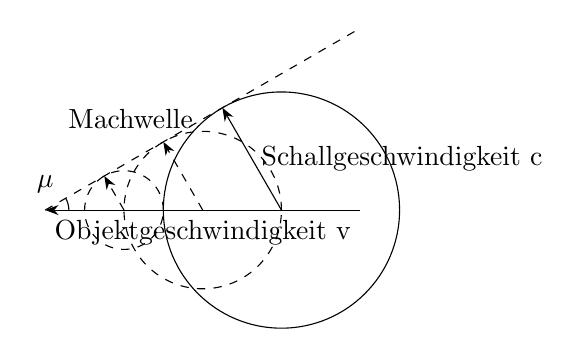
\begin{tikzpicture}
			
			\coordinate (OO) at (0,0);				
			
			% Circle centers
			\coordinate (P3) at (1,0);				
			\coordinate (P2) at (2,0);				
			\coordinate (P1) at (3,0);				
			
			% Tangential points
			\coordinate (S3) at ({1 *(1-sin(30)*sin(30)},{1*sin(30)*cos(30)});				
			\coordinate (S2) at ({2 *(1-sin(30)*sin(30)},{2*sin(30)*cos(30)});				
			\coordinate (S1) at ({3 *(1-sin(30)*sin(30)},{3*sin(30)*cos(30)});				
			
			% Endpoint of Mach front
			\coordinate (SX) at (4,{4*tan(30)});				
			
			\draw [-Stealth,dashed] (P3) -- node[above] {} (S3);
			\draw [-Stealth,dashed] (P2) -- node[above] {} (S2);
			\draw [-Stealth] (P1) -- node[right] {Schallgeschwindigkeit c} (S1);
			
			\coordinate (O) at (4,0);
			%		\coordinate (C) at (0,3);
			%		\coordinate (D) at ($(C)!(P3)!(B)$);
			
			\draw [-Stealth] (O) -- node[below] {Objektgeschwindigkeit v} (OO);
			\draw [dashed] (OO) -- node[left] {Machwelle} (SX);
			
			\pic [draw, angle radius=3mm, angle eccentricity=1.2mm] {angle = P3--OO--S3};
			\node[above = 0.1cm and 0.8cm of OO] {$\mu$};
			
			\dotMarkRightAngle[size=6pt](OO,S1,P1);
			
			\draw (P3) [dashed] circle ({1*sin(30)});
			\draw (P2) [dashed] circle ({2*sin(30)});
			\draw (P1) circle ({3*sin(30)});
			
			
		\end{tikzpicture}
		
	}		
	
	
	$M < 1.0$: Subsonic \\
	$M = 1.0$: Transonic \\
	$M > 1.0$: Supersonic \\
	$M > 5.0$: Hypersonic
	
\end{sectionbox}


% ======================================================================
% End
% ======================================================================
\end{document}
